% =============================================================================
% Pico Miner -- Proof of Concept Document
% FPGA-Based Proof of Work Mining Accelerator
% =============================================================================
\documentclass[12pt,a4paper]{article}

% --- Packages ---
\usepackage[utf8]{inputenc}
\usepackage[T1]{fontenc}
\usepackage[english]{babel}
\usepackage{geometry}
\usepackage{graphicx}
\usepackage{amsmath,amssymb}
\usepackage{listings}
\usepackage{xcolor}
\usepackage{hyperref}
\usepackage{booktabs}
\usepackage{caption}
\usepackage{algorithm}
\usepackage{algorithmic}
\usepackage{tikz}
\usetikzlibrary{shapes,arrows,positioning,fit}

\geometry{margin=2.5cm}

% --- Code listing style ---
\definecolor{codebg}{rgb}{0.95,0.95,0.95}
\definecolor{codegreen}{rgb}{0,0.5,0}
\definecolor{codegray}{rgb}{0.5,0.5,0.5}
\definecolor{codeblue}{rgb}{0.1,0.1,0.7}

\lstdefinestyle{cstyle}{
    backgroundcolor=\color{codebg},
    basicstyle=\ttfamily\footnotesize,
    breaklines=true,
    captionpos=b,
    commentstyle=\color{codegreen},
    keywordstyle=\color{codeblue}\bfseries,
    stringstyle=\color{red},
    numberstyle=\tiny\color{codegray},
    numbers=left,
    frame=single,
    language=C,
    showstringspaces=false,
    tabsize=4
}

% --- Title ---
\title{%
    \textbf{Pico Miner} \\[0.5em]
    \large FPGA-Based Proof of Work Mining Accelerator \\[0.3em]
    \large Proof of Concept Document
}
\author{Pico Miner Project}
\date{\today}

% =============================================================================
\begin{document}
\maketitle
\tableofcontents
\newpage

% =============================================================================
\section{Introduction}
% =============================================================================

Cryptocurrency mining is the process by which new transactions are verified
and added to the blockchain ledger. The core computational challenge is
known as \textbf{Proof of Work (PoW)}: miners must find a value (called a
\textit{nonce}) such that the hash of the block data concatenated with the
nonce produces a result that satisfies a certain difficulty condition ---
typically, the hash must be numerically less than a \textit{target} value.

In Bitcoin, this involves computing the \texttt{SHA-256} hash function
twice (double SHA-256) over an 80-byte block header while iterating over
a 32-bit nonce space. The difficulty target is adjusted so that, on average,
a valid nonce is found every 10 minutes across the entire network.

\textbf{Pico Miner} is a proof-of-concept project that demonstrates the
fundamental principles of PoW mining accelerated on an FPGA. Rather than
implementing the full SHA-256 algorithm (which is complex and
resource-intensive), we use a \textbf{custom lightweight hash function}
that preserves the essential properties needed for PoW while being
practical for implementation in Vivado HLS on a Zynq-7020 FPGA.

% =============================================================================
\section{Background: How Bitcoin Mining Works}
% =============================================================================

\subsection{The Blockchain}

A blockchain is a distributed, append-only ledger where each block contains:
\begin{itemize}
	\item A reference (hash) to the previous block
	\item A set of transactions
	\item A timestamp
	\item A \textit{nonce} value
\end{itemize}

\subsection{Proof of Work}

The PoW mechanism requires that:
\begin{equation}
	\text{Hash}(\text{block\_header} \,\|\, \text{nonce}) < \text{target}
\end{equation}

where $\|$ denotes concatenation and the \textit{target} is a threshold
derived from the current difficulty. Since cryptographic hash functions
behave as pseudo-random oracles, the only way to find a valid nonce is
by \textbf{brute-force iteration} --- trying nonce values one by one until
the condition is met.

\subsection{Why FPGAs?}

FPGAs offer several advantages for PoW mining:
\begin{itemize}
	\item \textbf{Parallelism}: Multiple hash computations can run
	      simultaneously in hardware
	\item \textbf{Pipelining}: The hash computation can be deeply pipelined
	      to achieve high throughput (one hash per clock cycle)
	\item \textbf{Energy efficiency}: Dedicated hardware is far more
	      energy-efficient than general-purpose CPUs or GPUs for this
	      repetitive computation
	\item \textbf{Low latency}: Direct hardware implementation avoids
	      instruction fetch/decode overhead
\end{itemize}

% =============================================================================
\section{Project Scope and Simplifications}
% =============================================================================

This project is a \textbf{proof of concept} designed for educational
purposes. The following table compares real Bitcoin mining with our
simplified implementation:

\begin{table}[h]
	\centering
	\caption{Comparison: Bitcoin Mining vs. Pico Miner}
	\begin{tabular}{@{}lll@{}}
		\toprule
		\textbf{Aspect} & \textbf{Bitcoin}                & \textbf{Pico Miner}                \\
		\midrule
		Hash function   & Double SHA-256 (512-bit blocks) & Custom 32-bit hash (PicoHash)      \\
		Block header    & 80 bytes (640 bits)             & 16 bytes (4 $\times$ 32-bit words) \\
		Nonce size      & 32 bits                         & 32 bits                            \\
		Difficulty      & 256-bit target comparison       & 32-bit target comparison           \\
		Output          & 256-bit hash                    & 32-bit hash                        \\
		Network         & Peer-to-peer blockchain         & Standalone demonstration           \\
		\bottomrule
	\end{tabular}
\end{table}

\subsection{What is Preserved}

Despite the simplifications, our project preserves the \textbf{core
	algorithmic structure} of PoW mining:
\begin{enumerate}
	\item \textbf{Brute-force nonce search}: The miner iterates through
	      nonce values, just like a real miner
	\item \textbf{Hash computation per nonce}: Each nonce attempt requires
	      a full hash computation
	\item \textbf{Difficulty-based acceptance}: The hash must be below
	      a target to be ``valid''
	\item \textbf{Hardware acceleration}: The hash + compare loop runs
	      in dedicated FPGA hardware, controlled by ARM software
	\item \textbf{HLS optimization}: We demonstrate how pipeline and
	      unroll directives dramatically improve throughput
\end{enumerate}

% =============================================================================
\section{PicoHash: Custom Hash Function}
% =============================================================================

\subsection{Design Rationale}

Our custom hash function, \textbf{PicoHash}, is inspired by the DJB2 and
FNV hash families. It is designed to be:
\begin{itemize}
	\item \textbf{Simple}: Easily synthesizable in HLS with minimal
	      resources
	\item \textbf{Deterministic}: Same input always produces the same
	      output
	\item \textbf{Avalanche-prone}: Small input changes cause large
	      output changes (desirable for PoW)
	\item \textbf{Non-invertible (practically)}: Difficult to reverse
	      analytically, requiring brute force to find a valid nonce
\end{itemize}

\subsection{Algorithm Definition}

\begin{algorithm}[H]
	\caption{PicoHash$(data[0..N{-}1], \, nonce)$}
	\begin{algorithmic}[1]
		\STATE $h \leftarrow \texttt{0x5A3C\_F1E7}$ \COMMENT{Initial seed}
		\FOR{$i = 0$ \TO $N-1$}
		\STATE $h \leftarrow h \oplus data[i]$ \COMMENT{XOR with data word}
		\STATE $h \leftarrow h \times \texttt{0x01000193}$ \COMMENT{FNV prime multiply}
		\STATE $h \leftarrow h \oplus (h \gg 16)$ \COMMENT{Mix upper bits into lower}
		\ENDFOR
		\STATE $h \leftarrow h \oplus nonce$ \COMMENT{Incorporate nonce}
		\STATE $h \leftarrow h \times \texttt{0x5BD1E995}$ \COMMENT{MurmurHash finalizer constant}
		\STATE $h \leftarrow h \oplus (h \gg 13)$
		\STATE $h \leftarrow h \times \texttt{0x5BD1E995}$
		\STATE $h \leftarrow h \oplus (h \gg 15)$
		\RETURN $h$
	\end{algorithmic}
\end{algorithm}

The algorithm has two phases:
\begin{enumerate}
	\item \textbf{Absorption}: Iterates over the block data words, mixing
	      each into the hash state via XOR and multiplication
	\item \textbf{Finalization}: After incorporating the nonce, applies
	      a MurmurHash-inspired bit-mixing sequence to ensure good
	      avalanche behavior
\end{enumerate}

\subsection{Properties}

\begin{itemize}
	\item \textbf{Output size}: 32 bits (unsigned integer)
	\item \textbf{Input}: Array of 32-bit words + 32-bit nonce
	\item \textbf{Latency}: $O(N)$ for $N$ data words, plus constant
	      finalization steps
	\item \textbf{Collision resistance}: Not cryptographically secure
	      (32-bit output), but sufficient for educational PoW demonstration
\end{itemize}

% =============================================================================
\section{System Architecture}
% =============================================================================

\subsection{Hardware/Software Partitioning}

The system follows the Zynq PS/PL architecture:

\begin{center}
	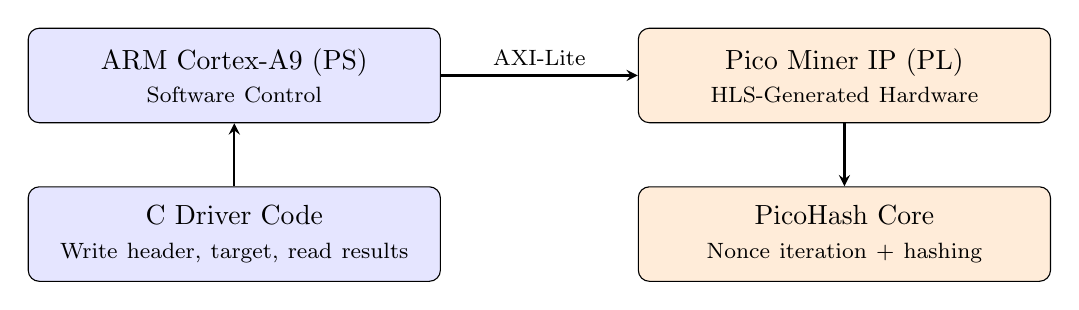
\begin{tikzpicture}[
			block/.style={rectangle, draw, fill=blue!10, text width=5cm,
					text centered, minimum height=1.2cm, rounded corners},
			hwblock/.style={rectangle, draw, fill=orange!15, text width=5cm,
					text centered, minimum height=1.2cm, rounded corners},
			arrow/.style={->, thick, >=stealth}
		]
		% PS side
		\node[block] (arm) {ARM Cortex-A9 (PS) \\ \footnotesize Software Control};
		\node[block, below=0.8cm of arm] (driver) {C Driver Code \\ \footnotesize Write header, target, read results};

		% PL side
		\node[hwblock, right=2.5cm of arm] (miner) {Pico Miner IP (PL) \\ \footnotesize HLS-Generated Hardware};
		\node[hwblock, below=0.8cm of miner] (hash) {PicoHash Core \\ \footnotesize Nonce iteration + hashing};

		% Connections
		\draw[arrow] (arm) -- node[above]{\footnotesize AXI-Lite} (miner);
		\draw[arrow] (driver) -- (arm);
		\draw[arrow] (miner) -- (hash);
	\end{tikzpicture}
\end{center}

\subsection{HLS IP Interface}

The HLS IP function signature is:

\begin{lstlisting}[style=cstyle]
void pico_miner(
    int block_header[4],   // Input: simplified block header
    int difficulty_target,  // Input: hash must be < this value
    int nonce_start,        // Input: beginning of nonce range
    int nonce_end,          // Input: end of nonce range
    int *found_nonce,       // Output: the winning nonce (if found)
    int *found_hash,        // Output: the winning hash value
    int *status             // Output: 1 = found, 0 = not found
);
\end{lstlisting}

All ports are mapped to AXI-Lite (\texttt{s\_axilite}) bundled into a
single bus called \texttt{myaxi}, following the same methodology as the
course examples.

\subsection{Mining Operation Flow}

\begin{enumerate}
	\item The ARM processor writes the block header (4 words), difficulty
	      target, and nonce range to the HLS IP via AXI-Lite registers
	\item The ARM issues \texttt{ap\_start} to begin computation
	\item The HLS IP iterates through the nonce range:
	      \begin{enumerate}
		      \item Computes $h = \text{PicoHash}(\text{header}, \text{nonce})$
		      \item If $h < \text{target}$: stores the nonce and hash, sets
		            status to 1, and terminates early
	      \end{enumerate}
	\item The ARM polls \texttt{ap\_done}, then reads the results
	\item If no valid nonce was found in the range, status is 0
\end{enumerate}

% =============================================================================
\section{HLS Optimization Strategy}
% =============================================================================

Following the course methodology, we explore multiple optimization levels:

\subsection{Solution 1: Baseline}
No directives applied. The nonce search loop executes sequentially with
no pipelining or parallelism.

\subsection{Solution 2: Loop Pipelining}
\begin{lstlisting}[style=cstyle]
#pragma HLS PIPELINE II=1
\end{lstlisting}
Applied to the main nonce search loop. This allows the next nonce
iteration to begin before the previous one completes, achieving an
\textbf{Initiation Interval (II) of 1} --- one new hash per clock cycle
after the pipeline fills.

\subsection{Solution 3: Array Partitioning}
\begin{lstlisting}[style=cstyle]
#pragma HLS ARRAY_PARTITION variable=block_header complete
\end{lstlisting}
Combined with loop pipelining, this ensures all block header words
can be read simultaneously, eliminating memory port bottlenecks.

\subsection{Expected Performance Scaling}

\begin{table}[h]
	\centering
	\caption{Expected Performance Across Solutions (estimated)}
	\begin{tabular}{@{}lccc@{}}
		\toprule
		\textbf{Solution}          & \textbf{Latency/Hash} & \textbf{II} & \textbf{Throughput} \\
		\midrule
		Baseline (no directives)   & $\sim$20 cycles       & $\sim$20    & $\sim$5 MH/s        \\
		Loop pipelining            & $\sim$20 cycles       & $\sim$1     & $\sim$100 MH/s      \\
		Pipeline + array partition & $\sim$10 cycles       & $\sim$1     & $\sim$100 MH/s      \\
		\bottomrule
	\end{tabular}
\end{table}

\noindent (At 100 MHz clock, II=1 yields $\sim$100 million hashes/second.)

% =============================================================================
\section{Verification Strategy}
% =============================================================================

\subsection{C Simulation (csim)}

A software testbench (\texttt{pico\_miner\_tb.cpp}) contains:
\begin{itemize}
	\item A \texttt{pico\_miner\_sw()} reference function implementing
	      the same algorithm in pure C
	\item Test cases with known difficulty levels and expected results
	\item Bit-exact comparison between SW and HW outputs
\end{itemize}

\subsection{C/RTL Co-Simulation (cosim)}

After C synthesis, the generated RTL is verified against the C testbench
using Vivado HLS co-simulation to confirm cycle-accurate correctness.

\subsection{ARM Integration Test}

The ARM driver code (\texttt{pico\_miner\_arm.c}) performs the same SW vs. HW
comparison on the actual Zynq hardware, printing results via UART.

% =============================================================================
\section{Conclusion}
% =============================================================================

Pico Miner demonstrates that the fundamental principles of cryptocurrency
Proof of Work mining can be effectively mapped to FPGA hardware using
Vivado HLS. By using a simplified hash function, we preserve the core
computational pattern --- brute-force nonce search with hash comparison ---
while keeping the design practical for a Zynq-7020 target.

The project showcases:
\begin{itemize}
	\item High-Level Synthesis of a mining algorithm from C to RTL
	\item AXI-Lite integration for PS/PL communication
	\item HLS directive optimization (pipeline, array partition)
	\item SW/HW verification methodology with golden model comparison
\end{itemize}

This approach could be extended to implement real SHA-256 hashing for
actual Bitcoin mining, though that would require significantly more
FPGA resources and design effort.

% =============================================================================
\end{document}
